\documentclass[12pt]{article}

\usepackage[english]{babel}
\usepackage[utf8]{inputenc}
\usepackage{amsmath}
\usepackage{amssymb}
\usepackage{graphicx}
\usepackage{geometry}
\usepackage[colorinlistoftodos]{todonotes}
\usepackage{caption}
    \captionsetup{font=small,labelfont=bf}
\usepackage{enumerate}
\usepackage{lscape}
\usepackage{caption}
\usepackage{verbatim}
\usepackage{csvsimple}

\captionsetup{font={small}}
\geometry{left=2.0cm, right=2.0cm, top=2.5cm, bottom=2.5cm}

\title{STAT601 Homework 1}

\author{Xingche Guo}

\date{\today}

\linespread{1.3}
\begin{document}
\maketitle

\section*{(1)}
For "Bliss Beetle Data" problem, define mortality rate $Y_i$ to be the response variable for each sample $i$. Define the natural logarithm of $CS_2$ dosage $X_i$ as covariate and $m_i$ as the total number of insects. Then we can use a generalized linear model with Binomial random component to fit the model, where $y_i \sim Binomial(m_i,p_i)$, then the marginal density of $y_i$ is:

 \begin{eqnarray*}
 f(y_i | m_i,p_i) &=&
\left(                        
\begin{matrix}
 m_i \\
m_i y_i 
\end{matrix}
\right)
p_i^{m_i y_i }(1-p_i)^{m_i (1-y_i)}, \\
&=& exp\{m_i \phi (y_i \theta_i - b(\theta_i))+log\left(                        
\begin{matrix}
 m_i \\
m_i y_i 
\end{matrix}
\right)\}.
\end{eqnarray*}

where:
$$\theta_i = log \frac{p_i}{1-p_i}; \ \ b(\theta_i)=-log \frac{e^{-\theta_i}}{1+e^{-\theta_i}}; \ \ \ \phi = 1.$$
We then can use the "basicglm" R function provided in STAT520 if we choose the link function to be logit function.\\
\\
 If we decide to use Pregibon's one-parameter link as a parameterized link function, where:
 $$g(\mu_i|\lambda)=\log\{   \frac{(1-\mu_i)^{-\lambda}-1}{\lambda}  \}$$
 Then:\\
Linear Predictor: 
$$\eta_i = \beta_0 + \beta_1 x_i$$
Mean (of $Y_i$):
$$\mu_i = 1 - \frac{1}{    \{  1 + \lambda \exp(\eta_i)  \}^{1/ \lambda}     }$$ 
Variance (of $Y_i$):
$$V(\mu_i)=\mu_i (1-\mu_i)$$


We can express the Fisher Scoring algorithm as follow (The detailed information can be found in STAT601 Notes p.11-p.18):
$$\xi^{(m+1)}=\xi^{(m)}+H^{-1}\nabla L |_{\xi = \xi^{(m)}}.$$
where:
$$\xi = (\beta^{T}, \lambda)^{T}; \ \ H=\phi X_{A}^{T}WX_{A}; \ \ \nabla L=\phi X_{A}^{T}W\pmb{z}.$$
In this case, $X_A$ is an $n \times (2+1)$ matrix with $i^{th}$ row: $\pmb{x}_{A,i}^{T}=(1,x_i,-\frac{\partial \eta_i}{\partial \lambda})$. $\pmb{z}=(z_1,\dots,z_n)^{T}$ where $z_i = (y_i-\mu_i)\frac{\partial \eta_i}{\partial \mu_i}$. W is an $n \times n$ diagonal matrix with element $w_i = m_i[(\frac{\partial \eta_i}{\partial \mu_i})^2 V(\mu_i)]^{-1}$.

where: 
$$\frac{\partial \eta_i}{\partial \mu_i} = \frac{\lambda}{(1-\mu_i)\{ 1 - (1-\mu_i)^{\lambda}  \}}$$
$$\frac{\partial \eta_i}{\partial \lambda} = \frac{-\log(1-\mu_i)}{1 - (1-\mu_i)^{\lambda}}-\frac{1}{\lambda}$$

Using the algorithm above:

\begin{tabular}{|c|cccc|}
\hline
 & Logit (Series 1) & Pregibon's (Series 1) & Logit (Series 2) & Pregibon's (Series 2)\\
 \hline
$\hat{\beta_0}$ & -60.53629 & -41.56327 & -58.58627 & -35.28984 \\
$\hat{\beta_1}$ & 14.84134 & 10.07396 & 14.35719 & 8.498555 \\
$\hat{\lambda}$ & NA & 0.1147058 & NA & -0.2348097 \\
LogLik & -89.93865 & -88.66497  & -95.5821 & -93.46143\\
\hline
\end{tabular}
\\

In order to compute the results from the second column, I use the MLE of $\pmb{\beta}$ in the glm model with logit link in Series 1 to be the starting value of $\pmb{\beta}$ and 1 as the starting value of $\lambda$. For Series 2 (results in the forth column), I just use the result in the second column as starting value.\\


In order to test whether the model with estimated link can fit the model statistically better than the simpler model with a fixed logit link, we can apply the likelihood ratio test ($df = 1$):
$$\Lambda = -2 (l_{reduce}^{(1)} - l_{full}^{(1)}) = -2 (-89.93865 + 88.66497 ) = 2.54737$$
$$p-value^{(1)}= 0.110478$$.

Similarly, we can compute the p-value for series 2: 
$$p-value^{(2)}= 0.03945084$$.

Alternatively, we can use Wald's theory to compute the $95\%$ confidence intervals for $\lambda$:  
$$CI_{\lambda} = \hat{\lambda} \pm 1.96\sqrt{H^{-1}_{(3,3)}}$$. 
$H^{-1}_{(3,3)}$ is the third diagonal element of $H^{-1}$. 
$$CI_{\lambda}^{(1)} = (-0.6214067,  0.8508183).$$
$$CI_{\lambda}^{(2)} = (-0.8117860  0.3421666).$$

Since the p-value of series 2 is less than 0.05 and the $95\%$ CI for $\lambda$ does not contain 1,  there is strong evidence to say that the model with estimated link performs better than the simpler one for series 2.\\
  For series 1, although the p-value is greater than 0.05, it's still small and at the same time, the $95\%$ CI for $\lambda$ also does not contain 1. Thus, there is some evidence that the model with estimated link is better.



\section*{(2)}
In this problem, we only consider the model with estimated link since we've already determined to apply the parameterized link function to both series 1 and 2. In other word, we need to test:
$$H_0: \pmb{\beta}^{(1)}=\pmb{\beta}^{(2)}, \lambda^{(1)}=\lambda^{(2)}; \ \ \ \ \ \  H_1: (\pmb{\beta}^{(1)},\lambda^{(1)})^{T} \neq (\pmb{\beta}^{(2)},\lambda^{(2)})^{T}$$ 
Where $\pmb{\beta}^{(i)}$ and $\lambda^{(i)}$ denote the parameter for series $i$ in the glm model with estimated link.

It's easy to know that the log likelihood for the full model is:
$$l_{full}= l_{full}^{(1)}+ l_{full}^{(2)} = -88.66497 -93.46143 = -182.1264$$
$l_{full}^{(1)}$ and $l_{full}^{(2)}$ are the log likelihood function for series 1 and 2.

To compute the $l_{reduce}$, we only need to combine the data from two series and apply the same Fisher Scoring algorithm in problem 1:
$$l_{reduce}=-182.3305$$

We then apply the likelihood ratio test to compute the p value, the p value is 0.9385225. (df = 3).
Hence we conclude that there is not significant difference between the two series.


\section*{(3)}
By problem 1 and 2, we've found that the final model should be the model with estimated link which combine the data from two series.  Some estimates for the data are given below:\\

\begin{tabular}{|c|c|c|c|c|}
\hline
 $\hat{\beta_0}$ & $\hat{\beta_1}$ & $\hat{\lambda}$ & fitted LogLik & saturated LogLik\\
 \hline
-39.710772 & 9.608419 & 0.01197646  & -182.3305 & -178.192\\
\hline
\end{tabular}
\\

(I use the MLE of $(\pmb{\beta},\lambda)$ from the estimated link model in series 1 as starting value.)\\

To compute the $90\%$ confidence interval for $\mu(x)$, we need to apply the Wald's theory and Delta's method:
$$CI_{\mu} = \hat{\mu(x)} \pm z_{0.95} \sqrt{D^{T}H^{-1}D}$$
Where $z_{0.95}$ is the 0.95 quantile of $Normal(0,1)$, $D=(\frac{\partial \mu(x)}{\partial \beta_0},\frac{\partial \mu(x)}{\partial \beta_1},\frac{\partial \mu(x)}{\partial \lambda})^{T}|_{(\pmb{\beta},\lambda)=(\pmb{\hat{\beta}},\hat{\lambda})}$.

$$\frac{\partial \mu(x)}{\partial \beta_0}=\frac{\exp(\eta)}{(1+\lambda \exp(\eta))^{1+\frac{1}{\lambda}}}$$
$$\frac{\partial \mu(x)}{\partial \beta_1}=\frac{x \exp(\eta)}{(1+\lambda \exp(\eta))^{1+\frac{1}{\lambda}}}$$
$$\frac{\partial \mu(x)}{\partial \lambda} = -\exp\{-\frac{1}{\lambda}\log(1+\lambda \exp(\eta))\}
\{-\frac{1}{\lambda} \frac{\exp(\eta)}{1+\exp(\eta)) \lambda} +  \frac{\log(1+\exp(\eta)\lambda)}{\lambda^2} \}$$

Where $\eta=\eta(x)=\beta_{0}+\beta_{1}x$. So, we can plot the $90\%$ pointwise confidence band in figure 1.

\begin{figure}[h] 
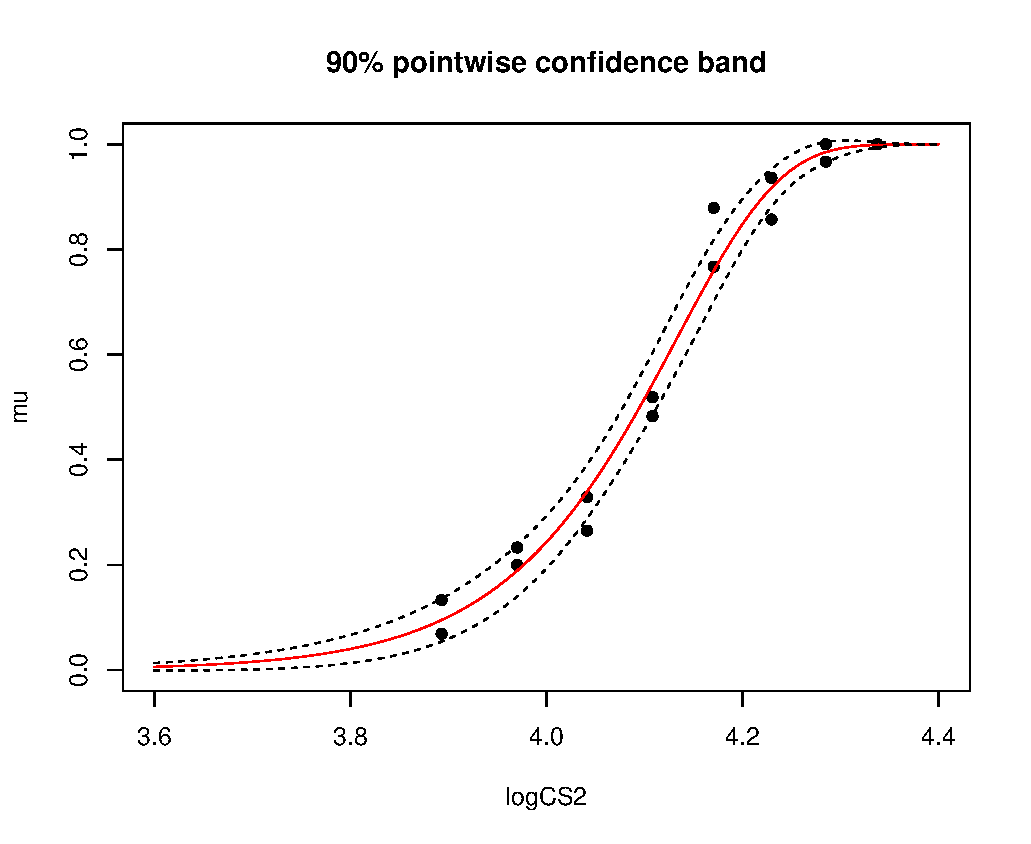
\includegraphics[width=1.0\textwidth]{Rplot1.pdf}
\caption{}
\end{figure}

For tolerance distribution:
$$G(x|\lambda, \pmb{\beta}) = \mu(x) = 1 - \frac{1}{(\lambda \exp(\beta_0 + \beta_1 x)+1)^{1/\lambda}}$$
By differentiation, we have the tolerance density function:
$$g(x|\lambda, \pmb{\beta}) = \frac{\beta_1 \exp(\beta_0 + \beta_1 x)}{(1 + \lambda \exp(\beta_0 + \beta_1 x))^{1+\frac{1}{\lambda}} }$$

Thus, we can draw the estimated tolerance density $g(x|\hat{\lambda}, \pmb{\hat{\beta}})$ in figure 2.

\begin{figure}[h] 
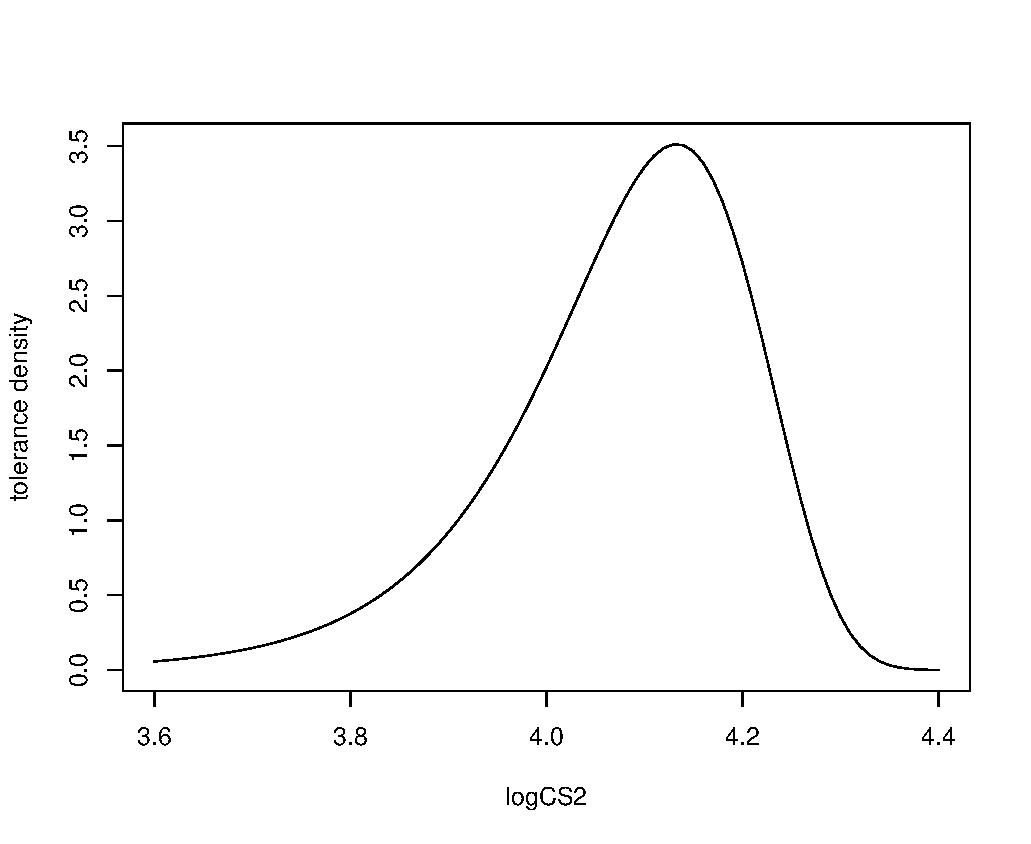
\includegraphics[width=1.0\textwidth]{Rplot2.pdf}
\caption{}
\end{figure}


\section*{(4)}
\begin{figure}[h] 
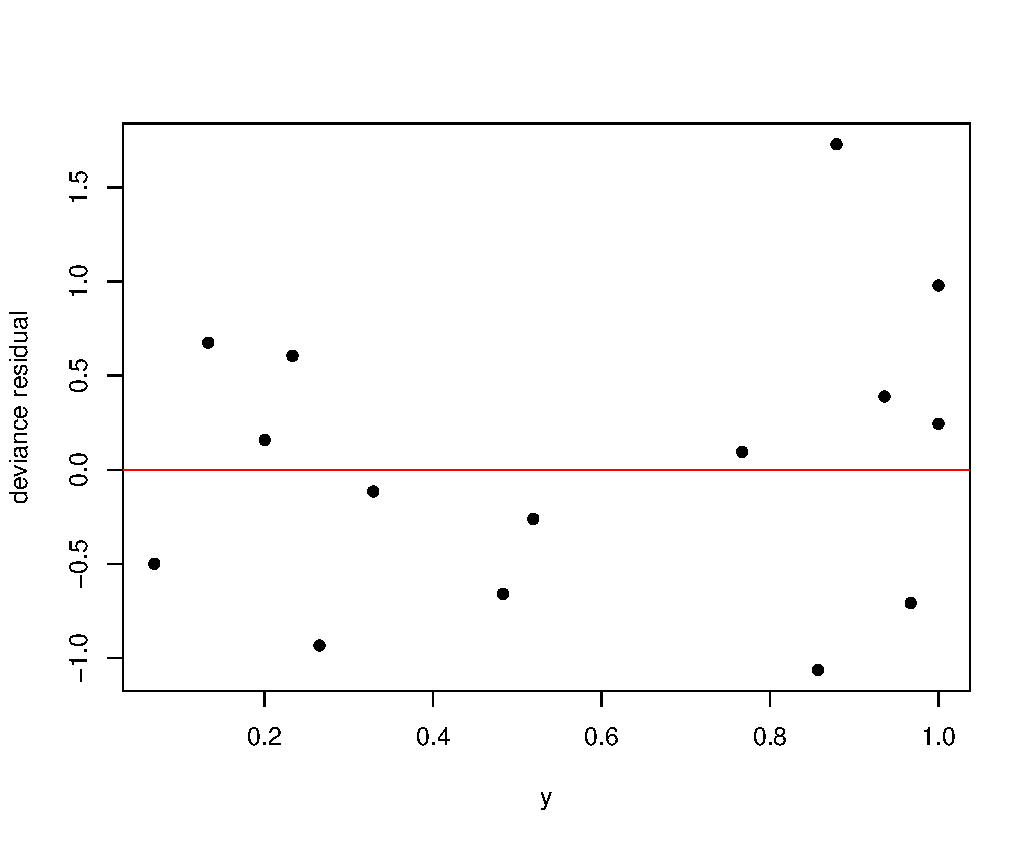
\includegraphics[width=1.0\textwidth]{Rplot3.pdf}
\caption{}
\end{figure}

We can plot the deviance residuals against fitted value in figure 3.  I notice that there isn't any obvious pattern in this plot. Furthermore, we can assess the model by likelihood ratio test. (compare fitted model to saturated model)

$$-2(l_{fit} - l_{sat}) \sim \chi^{2}_{15-3}$$
$$ l_{sat}= \sum_{i=1}^{n}  \{ m_i  (y_i \log(\frac{y_i}{1-y_i}) + \log(1-y_i) ) + c(y_i) \}$$
$$ l_{fit}= \sum_{i=1}^{n}  \{ m_i  (y_i \log(\frac{\hat{\mu_i}}{1-\hat{\mu_i}}) + \log(1-\hat{\mu_i}) ) + c(y_i) \}$$

The p value of this test is 0.7631181, which implies the fitted model can fit the data well.




\section*{(5)}
For the glm for logit link funciton, I use basicglm provided in STAT520.
For the glm for parameterized link function, I have written the Fisher Scoring algorithm in R.




\end{document}